\documentclass{beamer}
\usetheme{Madrid}
\usepackage{tikz}

\newcommand{\F}{\mathbb{F}}
\newcommand{\B}{\mathcal B}
\newcommand{\HH}{\mathcal H}
\newcommand{\RR}{\mathcal R}
\newcommand{\cl}{\operatorname{cl}}
\newcommand{\si}{\operatorname{si}}
\newcommand{\PG}{\operatorname{PG}}
\newcommand{\Aut}{\operatorname{Aut}}

\title{Sample title}
\author{Anonymous}
%\institute{Overleaf}
\date{2026}

\begin{document}

\frame{\titlepage}

\begin{frame}
\frametitle{Basic concepts}
\begin{itemize}
  \item A \emph{matroid} is a finite ground set $E$ with a family
    $\mathcal I$ of independent subsets. The empty set is independent,
    subsets of independent sets are independent, and if $I,J\in\mathcal I$
    with $|I|<|J|$, some $j\in J\setminus I$ makes $I\cup\{j\}$ independent.
  \item A canonical example is a \emph{vector matroid}. Its elements
    label the columns of a matrix, and its independent sets label
    sets of linearly independent columns.
  \item Some matroids have no matrix representation. A matroid that
    can be represented by a matrix over a field $\F$ is called
    $\F$-representable.
  \item We need a few more concepts to state the problem. We omit detailed
    proofs due to time constraints.
\end{itemize}
\end{frame}

\begin{frame}
  \begin{itemize}
    \item Analogous concepts from linear algebra still carry over.
      \begin{itemize}
        \item A basis is a maximal independent set.
        \item All bases have the same size, called the rank.
      \end{itemize}
    \item We often describe matroids using a labelled ground set and a set
      of bases, e.g. $E=\{0, 1, 2\}$, $\B = \{\{1, 2\}, \{0, 2\}\}$.
    \item The dual $M^*$ has the same ground set as $M$ and bases
      $\{E\setminus B:B\in\B(M)\}$.
    \item Two fundamental operations give minors.
      \begin{itemize}
        \item Deletion $M\setminus T$ has ground set $E\setminus T$.
          Its independent sets are the independent sets of $M$ contained
          in $E\setminus T$.
        \item Contraction by $T\subseteq E$ is $M/T = (M^*\setminus T)^*$.
      \end{itemize}
  \end{itemize}
\end{frame}

\begin{frame}
  \frametitle{Problem statement}
  \begin{itemize}
    \item We classified all rank-$4$, $11$-element excluded minors for
      $\F_5$-representability up to isomorphism.
    \item We call an $\F_5$-representable matroid a \emph{quinary} matroid.
    \item An \emph{excluded minor for $\F_5$-representability} is a
      nonquinary matroid $M$ such that both $M/e$ and $M\setminus e$ are
      quinary for every $e\in E(M)$.
    \item These are the minimal nonquinary matroids under the minor relation.
    \item The study of excluded minors is extremely important in matroid theory.
  \end{itemize}
\end{frame}
\begin{frame}
  \frametitle{Comparison of methodology}
  \begin{itemize}
    \item We used an LLM to solve the problem.
    \item Directly asking the question left the classification incomplete.
    \item We completed the classification by giving the LLM access to
      computational tools for an exhaustive search.
  \end{itemize}
\end{frame}
\begin{frame}
  \frametitle{Proof outline}
  \begin{itemize}
    \item The proof can be broken down into a few steps.
    \item The broad idea is to view an $11$-element excluded minor $M$ as
      an extension of a $10$-element quinary matroid $N=M\setminus e$.
    \item For each $N$, we want extensions $M$ which are nonquinary but
      all of whose deletions and contractions are quinary.
    \item First generate all appropriate $N$.
    \item Then enumerate all nonquinary $M$ whose deletions are quinary.
      To do this, list the quinary extensions by $e$ of $N$ and of
      $N\setminus f$ for every $f\in E(N)$.
    \item Finally, pick those for which all single-element contractions are
      quinary. Then deduplicate up to isomorphism.
  \end{itemize}
  We shall give a bit more detail for each step, especially the computations involved.
\end{frame}

\begin{frame}
  \frametitle{Step 1}
  Generate $10$-element quinary matroids. Due to a key result, we only
  need connected simple rank-$4$ ones up to isomorphism.

  We say that two matrices over $\F_5$ are \emph{field-isomorphic} if they
  differ by invertible row operations, nonzero column scalings and a
  column permutation.
  \begin{itemize}
    \item First generate the corresponding matrices up to field isomorphism.
      Start with $I_4$ by reducing a basis to the identity. By simplicity,
      it suffices to append unused projective points, one nonzero vector
      per one-dimensional subspace.
    \item Separately, obtain their labelled basis representations and
      deduplicate them up to matroid isomorphism.
    \item Sage provides methods to check field isomorphism and matroid
      isomorphism.
  \end{itemize}
\end{frame}
\begin{frame}
  \frametitle{Step 2}
  Generate the candidate extensions for the contraction tests.

  \par Let $P=\{0,\dots,9\}$ and take a new label $e=10$. We work with
  labelled matroids, whose bases are subsets of a fixed ground set.
  Let $\mathcal P$ contain one labelled representative on $P$ of each
  connected simple rank-$4$ quinary matroid on $10$ elements.

  \par Let $\mathcal D(N)$ be the set of simple rank-$4$ matroids $M$ on
  $P\cup\{e\}$ with $M\setminus e=N$, with $M$ nonquinary, and with
  $M\setminus a$ quinary for every $a\in P\cup\{e\}$.

  \par We keep all labelled members of $\mathcal D(N)$.
  Our goal in this step is to exhaust $\mathcal D(N)$ for all
  $N\in\mathcal P$.
  \par As mentioned before, we do this by enumerating extensions.
\end{frame}
\begin{frame}
  We first describe how to encode extensions.
  \begin{itemize}
    \item Let $N\in\mathcal P$ and suppose $M\setminus e=N$. For a rank-$4$
      extension $M$, the unknown bases are of the form $T\cup\{e\}$
      for triples $T\subseteq P$. Set $x_T=1$ exactly when this set
      is a basis. An arbitrary $x$ need not define a matroid.
    \item Let $\pi_f(x)$ restrict $x$ to triples avoiding $f$. This
      gives the additional basis data for $M\setminus f$.
    \item Let $\RR(Q)$ be the set of bit rows on triples of $E(Q)$
      for simple rank-$4$ quinary extensions of $Q$ by $e$.
      \begin{itemize}
        \item $x\in\RR(N)$ gives a quinary extension of $N$.
        \item $\pi_f(x)\in\RR(N\setminus f)$ gives a simple rank-$4$
          quinary deletion at $f$.
      \end{itemize}
    \item If all deletion rows are allowed, the full family defines a
      simple matroid. Any two proposed bases use at most eight labels,
      so basis exchange holds in a common deletion. Every pair of
      elements also survives in a simple deletion.
    \item The assignments corresponding exactly to $\mathcal D(N)$ are
      \[
        \mathcal S(N)=
        \{x:\pi_f(x)\in\RR(N\setminus f)\text{ for every }f\in P\}
        \setminus\RR(N).
      \]
  \end{itemize}
\end{frame}
\begin{frame}
  \frametitle{Step 2.1}
  For $Q=N$ or $Q=N\setminus f$, a labelled representation is a
  matrix over $\F_5$ with one column per element of $Q$. Its linearly
  independent column sets give the independent sets of $Q$. Two are labelled
  projectively equivalent if invertible row operations and nonzero
  column scalings relate them with the labels fixed.

  We generate $\mathcal L(Q)$, one matrix per labelled projective
  equivalence class, as follows.
  \begin{itemize}
    \item For each field-isomorphism class in the catalogue whose matroid
      is isomorphic to $Q$, choose one matrix and relabel its columns
      using an isomorphism to $Q$. Then apply all automorphisms of $Q$
      to the column labels.
    \item Deduplicate the resulting matrices up to labelled projective
      equivalence by normalisation.
  \end{itemize}
\end{frame}

\begin{frame}
  \frametitle{Step 2.1: computations}
  To compute $\Aut(Q)$, construct a coloured bipartite graph.
  \begin{itemize}
    \item Each element is a blue vertex and each basis is a red vertex.
    \item Connect a blue vertex to a red vertex exactly when the element
      belongs to the basis.
    \item The colour-preserving graph automorphisms, which Sage can compute,
      induce exactly $\Aut(Q)$ on the element vertices.
  \end{itemize}
\end{frame}
\begin{frame}
  For normalisation, first fix an ordered basis $B$ and use Gaussian
  elimination to make its columns $I_r$. Let the remaining columns
  form $Z$. The basis data of $Q$ determine which $Z_{ij}$ are
  nonzero. Blocks $Z$ and $Z'$ obtained from labelled projectively
  equivalent matrices can only differ by row and column scalings.

  Consider a bipartite support graph.
  \begin{itemize}
    \item Each row of $Z$ gives a vertex on one side and each column
      of $Z$ gives a vertex on the other side.
    \item Connect row $i$ to column $j$ exactly when $Z_{ij}\ne0$.
    \item Fix a spanning tree in each component.
    \item In each tree, fix the root multiplier at $1$ and choose the
      remaining multipliers to make every tree entry $1$. This gives a
      unique normalised block for the equivalence class.
  \end{itemize}
\end{frame}

\begin{frame}
  \frametitle{Step 2.2}
  Build $\RR(Q)$.

  \par Let $V\in\mathcal L(Q)$ and let $v$ represent an unused
  projective point. The matrix $[V\mid v]$ represents a simple rank-$4$
  quinary extension of $Q$ by $e$. Its row is
  \[
    z_T=\mathbf 1\!\left\{\det[\,V_T\mid v\,]\ne0\right\},
    \qquad T\in\binom{E(Q)}3.
  \]
  The distinct rows over all such $V$ and $v$ are exactly $\RR(Q)$.

  \par For each $V$, we compute the determinant tests in one shot.
  Expand along $v$ to write each determinant as $c_T^{\mathsf T}v$.
  Stack the cofactor rows in $C$ and the projective point columns in
  $D$. The product $CD$ over $\F_5$ gives all the tests at once.
\end{frame}

\begin{frame}
  \frametitle{Step 2.3}
  Compressing the representation.
  \begin{itemize}
    \item Right now, entries in $\RR(Q)$ are recorded with a bit for
      each triple $T\subseteq E(Q)$, in lexicographic order.
    \item Dependent triples have bit $0$. Independent triples
      spanning the same hyperplane have equal bits, so we can use
      one bit per hyperplane.
    \item Let $\HH(N)$ be the hyperplanes of $N$ and let
      \[
        C_f=\{\cl_N(T):T\in\binom{P\setminus\{f\}}3,\ r_N(T)=3\}
      \]
      be the hyperplanes spanned by triples surviving deletion of $f$.
      Let $A_f$ be $\RR(N\setminus f)$ compressed to $C_f$ and
      let $A$ be $\RR(N)$ compressed to $\HH(N)$.
    \item We get a compressed version of $\mathcal S(N)$,
      \[
        \widehat{\mathcal S}(N)=
        \{y\in\{0,1\}^{\HH(N)}:y|_{C_f}\in A_f
          \text{ for every }f\in P\}\setminus A.
      \]
  \end{itemize}
\end{frame}

\begin{frame}
  \frametitle{Step 2.4}
  Produce the table for $\widehat{\mathcal S}(N)$. We want to combine
  the requirements $A_f$ for all $f\in P$ and remove the rows in $A$.
  This can be done in two ways.

  \medskip
  \textbf{Natural join}
  \begin{itemize}
    \item This is analogous to a database operation.
    \item A row of $A_{f_1}$ and a row of $A_{f_2}$ combine into a
      single assignment precisely when they agree on
      $C_{f_1}\cap C_{f_2}$.
    \item Build the full table for all columns in $\HH(N)$ by joining
      the tables $A_f$ one by one.
    \item Then remove rows that also appear in $A$.
  \end{itemize}
\end{frame}
\begin{frame}
  An alternative is to use SAT. Use one Boolean variable $y_H$ for
  each column in $\HH(N)$.
  \begin{columns}[T,onlytextwidth]
    \begin{column}{0.60\textwidth}
      \begin{enumerate}
        \item Encode each $A_f$ as a binary decision diagram and
          require its root to accept.
        \item Block each row of $A$.
        \item Record and block each solution until UNSAT.
      \end{enumerate}
    \end{column}
    \begin{column}{0.37\textwidth}
      \centering
      \small Example table $\{00,01,11\}$

      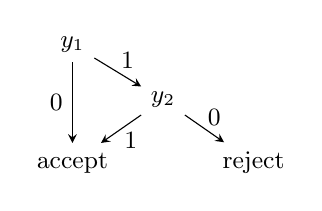
\begin{tikzpicture}[>=stealth,every node/.style={font=\small}]
        \node (first) at (0,0) {$y_1$};
        \node (second) at (1.15,-0.70) {$y_2$};
        \node (accept) at (0,-1.50) {accept};
        \node (reject) at (2.30,-1.50) {reject};
        \draw[->] (first) -- node[left] {$0$} (accept);
        \draw[->] (first) -- node[above right,inner sep=1pt] {$1$} (second);
        \draw[->] (second) -- node[below right,inner sep=1pt] {$1$} (accept);
        \draw[->] (second) -- node[above right,inner sep=1pt] {$0$} (reject);
      \end{tikzpicture}
    \end{column}
  \end{columns}

  \medskip
  At a node testing $y_H$, let $v$ be its value and $\ell,h$ the
  values of its $0,1$ branches. Its equivalence and four clauses are
  \[
    \begin{gathered}
      v\leftrightarrow((\neg y_H\land\ell)\lor(y_H\land h))\\[3pt]
      (\neg v\lor y_H\lor\ell),\qquad(\neg v\lor\neg y_H\lor h),\\
      (v\lor y_H\lor\neg\ell),\qquad(v\lor\neg y_H\lor\neg h).
    \end{gathered}
  \]
  To block a full row $a$, add $\bigvee_{H\in\HH(N)}(y_H\ne a_H)$.
\end{frame}

\begin{frame}
  \frametitle{Step 3}
  Check which elements of $\mathcal D(N)$ have all single-element
  contractions quinary.
  \begin{itemize}
    \item Every single-element contraction of a simple rank-$4$ matroid
      has rank $3$, and it suffices to check the simplifications of
      these contractions.
    \item Rank-$3$ simple quinary matroids can be enumerated as in
      Step~1. Check each simplification against the resulting catalogue.
    \item The members of $\mathcal D(N)$ with all these contractions quinary
      are the excluded minors. We deduplicate them up to isomorphism
      using Sage.
  \end{itemize}
\end{frame}

\begin{frame}
  \frametitle{Future work}
  We plan to complete the classification on $11$ elements across all
  ranks. By duality and existing work, it suffices to settle rank $5$.
\end{frame}

\end{document}
